\subsection{UC5 - Visualizzazione grafico di qualità delle previsioni}
\begin{figure}[H]
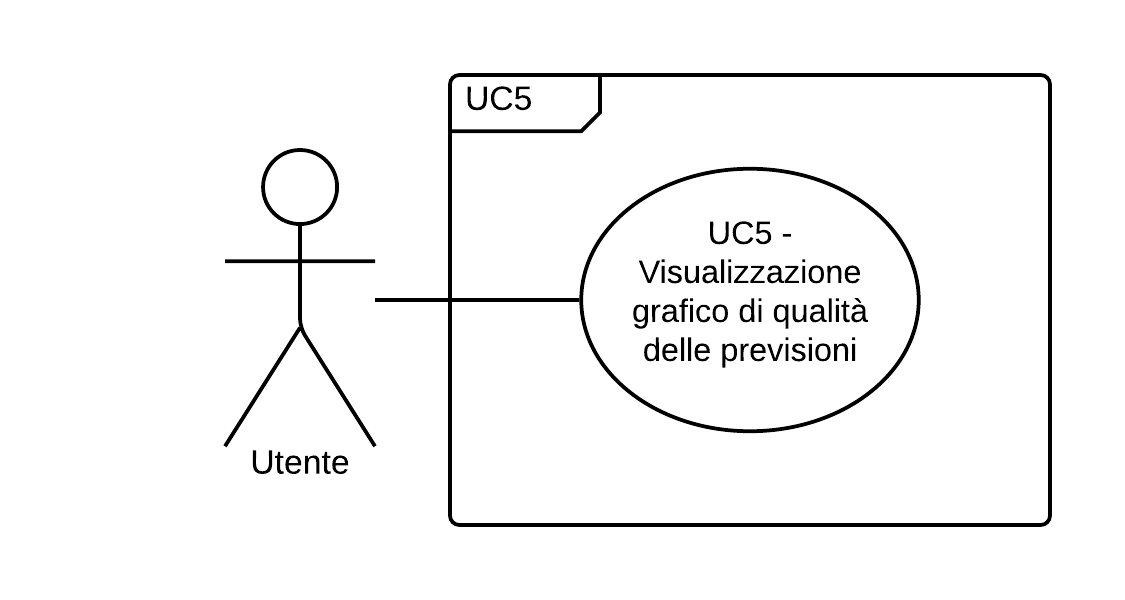
\includegraphics{img/UC5_-_Visualizzazione_grafico_di_qualita_delle_previsioni.png}
\caption{Diagramma degli use case di UC5}
\end{figure}
\begin{itemize}
	\item \textbf{Codice identificativo}: UC5;
	\item \textbf{Titolo}: visualizzazione grafico di qualità delle previsioni;
	\item \textbf{Attori primari}: utente;
	\item \textbf{Descrizione}: l'utente vuole visualizzare il grafico della qualità delle previsioni sui dati forniti;
	\item \textbf{Precondizioni}: l'addestramento è stato eseguito con l'applicazione esterna a Grafana\glo;
	\item \textbf{Postcondizioni}: l'utente ha visualizzo il grafico di qualità delle previsioni;
	\item \textbf{Scenario principale}: l'utente visualizza il grafico di qualità delle previsioni.
\end{itemize} 
